\documentclass[unnumsec,webpdf,contemporary,large]{oup-authoring-template}%
%\onecolumn % for one column layouts

%\usepackage{showframe}
\usepackage[T1]{fontenc}
\usepackage[utf8x]{inputenc}
\usepackage[french]{babel}
\usepackage{color}
\usepackage{appendix}

\usepackage[
  type={CC},
  modifier={by-nc-sa},
  version={3.0},
]{doclicense}

\usepackage{minted}
\setminted{encoding=utf-8,
            frame=lines,
            linenos}

\definecolor{dkgreen}{rgb}{0,0.6,0}
\definecolor{gray}{rgb}{0.5,0.5,0.5}
\definecolor{mauve}{rgb}{0.58,0,0.82}

\graphicspath{{Fig/}}

% line numbers^
%\usepackage[mathlines, switch]{lineno}
%\usepackage[right]{lineno}

\theoremstyle{thmstyleone}%
\newtheorem{theorem}{Theorem}%  meant for continuous numbers
%%\newtheorem{theorem}{Theorem}[section]% meant for sectionwise numbers
%% optional argument [theorem] produces theorem numbering sequence instead of independent numbers for Proposition
\newtheorem{proposition}[theorem]{Proposition}%
%%\newtheorem{proposition}{Proposition}% to get separate numbers for theorem and proposition etc.
\theoremstyle{thmstyletwo}%
\newtheorem{example}{Example}%
\newtheorem{remark}{Remark}%
\theoremstyle{thmstylethree}%
\newtheorem{definition}{Definition}

%============================== vector stuffs ==================================
\def\u{\vec{u}} % speed of the fluid
\def\r{\vec{r}} % space
\def\vnabla{\vec{\nabla}} %vectorial nabla
\def\F{\vec{F_{\text{ext}}}} % extrnal forces
\def\v{\vec{v}} % speed of the particles
\def\ei{\vec{e}_i} %speed of the lattices

%=========================== Mathematical Functions ============================
\newcommand\pderiv[3][1]{ %partial diferential
  \ifnum #1=1
    \dfrac{\partial #2}{\partial #3}
  \else
    \dfrac{\partial^{#1} #2}{{\partial #3}^{#1}}
  \fi 
}

%=============================== Math misc =====================================
\def\R{\mathbb{R}} %Real set
\def\feq{f^{\text{eq}}} %density probability distribution at equilibrium
\def\dl{\delta_l} 
\def\dt{\delta_t} 
\def\f{f_i}
\def\Re{\text{Re}}
\def\w{w_i}
\def\sign#1{\text{sign}(#1)}
%================================= Words =======================================
\def\NS{Navier-Stokes}

%================================== Command ====================================
\newcommand{\itemb}{\item[\textbullet ~]}

\license{\doclicenseImage \hfill Ce travail et disponible sous license
         Attribution-NonCommercial-ShareAlike (CC BY-NC-SA 3.0)}

\begin{document}
\journaltitle{Physique Numérique - Projet -  MU4PY108}
\DOI{\href{https://doi.org/10.5281/zenodo.4309974}{10.5281/zenodo.4309974}}
\copyrightyear{2020}
\pubyear{2020}
\access{18 Décembre 2020}
\appnotes{Compte rendus du projet de physique numérique}

\firstpage{1}


\title[LBM]{Implémentation et étude de la méthode de Boltzmann sur réseau en \sc{Fortran}}

\author[1,$\ast$]{\hypertarget{authors}{Yohan Duarte}}

\authormark{Y. Duarte et al.}

\address[1]{Étudiant en M1 PFA à Sorbonne Universitée, aka \href{https://github.com/Pacidus}{Pacidus}}

\corresp[$\ast$]{Me contacter. \href{email:pacidus@gmail.com}{pacidus@gmail.com}}

\abstract{La résolution des équations \NS{} constituent aujourd'hui un enjeu majeur dans de nombreux domaines.
Dans le cadre du projet de L'UE de Physique numérique, nous avons eu l'occasion d'implémenter la méthode de Boltzmann sur
réseau.
Cette méthode de résolution des équations de \NS{} constitue un changement de paradigme par rapport aux méthodes plus 
classiques.}

\keywords{\NS, méthode lattice Boltzmann, Bhatnagar-Gross-Krook, dynamique des fluides, Projet Numérique}

\maketitle

  \section{Introduction} \label{seq:intro}
    \paragraph*{}
  Des plasmas qui composent les nébuleuses aux arrivées d'eau de nos maisons en passant par les systèmes de
  refroidissement des centrales nucléaires et le flux sanguin alimentant notre métabolisme.
  Les fluides composent la majorité de la matière visible dans notre univers \cite{plasma}.
  La dynamique de ces fluides sont décrits par une équation rédigée au milieu XIXe siècle \cite{wiki:NS}.
  Fruit de la collaboration de générations de physiciens, les équations de \NS{} sont toujours aujourd'hui au cœur de
  nombreuses problématiques.
  La question de l'existence et de la régularité des solutions des équations de \NS{} en 3D constitue encore aujourd'hui 
  un problème ouvert et est l'un des problèmes du prix du millénaire de l'institut de mathématique de Clay 
  \cite{wiki:Mil}.

\paragraph*{}
  À défaut d'une solution analytique, c'est dès la première moitié du XXe siècle que les physiciens développent les
  premières méthodes de résolutions numériques des équations de \NS{} \cite{Hunt1998}.
  Depuis l'apparition des premiers ordinateurs, on a assisté à l'émergence de nombreuses méthodes numériques de résolution 
  de dynamique des fluides.
  La branche de la physique utilisant et étudiant ces méthodes et nommée \emph{Computational fluid dynamic} aussi abrégée 
  en CFD.
  La méthode qui nous intéresse ce nome la méthode de Boltzmann sur réseau plus couramment abrégée par LBM pour 
  \emph{Lattice Boltzmann Methods}.

\paragraph*{}
  Les LBM apparaissent au milieu des années 1980 \cite{D'HUMIERES1985, d_Humi_res_1986, PhysRevLett.56.1505, 
  DHUMIERES2009821} depuis lors cette méthode gagne en popularité comme l'illustre les 
  figures\footnote{La méthodologie permettent d'obtenir ces valeurs est critiquable néanmoins elles montrent une tendance 
  générale.} \ref{fig:LBM}, \ref{fig:CFD} et \ref{fig:ratio}.

\begin{figure}[htp]
  \center
  \includegraphics[width=\linewidth]{LBM} 
  \caption{Évolution du nombre de publication référencée dans \href{https://scholar.google.fr/}{Google Scholar} 
              possédant l'occurence <<Lattice Boltzmann Methods>> au cours de ces 30 dernières années.}
  \label{fig:LBM}
\end{figure}

\begin{figure}[htp]
  \center
  \includegraphics[width=\linewidth]{CFD} 
  \caption{Évolution du nombre de publication référencée dans \href{https://scholar.google.fr/}{Google Scholar} 
              possédant l'occurence <<Computational fluid dynamics>> au cours de ces 30 dernières années.}
  \label{fig:CFD}
\end{figure}

\begin{figure}[htp]
  \center
  \includegraphics[width=\linewidth]{LBMoCFD} 
  \caption{Rapport en pourcentage entre la figure \ref{fig:LBM} et la figure \ref{fig:CFD}.}
  \label{fig:ratio}
\end{figure}
  
  Ce succès peut s'expliquer par le fait que les LBM profitent de différentes propriétés intéressantes :
  \begin{itemize}
    \itemb Polyvalence :\\
    \emph{Les LBM peuvent être utilisées sur des problèmes très différents (aérodynamiques, médicaux, \dots{}).}

    \itemb Complexité :\\
    \emph{Les LBM peuvent facilement simuler des objets a géométries complexes et peuvent inclure des interactions entre
    plusieurs fluides ainsi que de la thermodynamique et d'autres forces en tout genres.}

    \itemb Parallélisation:\\
    \emph{Les LBM profitent de pleinement des accélérations permises par les architectures 
    \href{https://fr.wikipedia.org/wiki/Microprocesseur_multi-c\%C5\%93ur}{multicores} et 
    \href{https://fr.wikipedia.org/wiki/Processeur_graphique}{GPU} les simulations peuvent donc être déployées sur 
    différents \href{https://fr.wikipedia.org/wiki/Superordinateur}{HPC} et
    \href{https://fr.wikipedia.org/wiki/Grappe_de_serveurs}{clusters de calculs}.}
    
    \itemb Pas d'inconnues:\\
    \emph{Les LBM contrairement a d'autres méthodes plus communes résolvant directement \NS{} possède toutes les quantités
    nécessaires à la résolution déjà définies\footnote{Elle ne demande donc pas (par exemple) de résoudre les équations de
    poissons pour la pression à chaque itération.} et ce de manière locale\footnote{Ce qui explique le fait que les LBM 
    sont hautement parallélisable.}.}
  \end{itemize}
  
   Il est à noter que ces qualités sont inhérentes aux LBM et ne demandes pas de modifications majeures pour êtres 
   implémentées\footnote{À comprendre que l'algorithme de résolution reste le même.}.
   
  
  \section{Fluides, Macro, Micro et Méso} \label{seq:3M}
    \paragraph*{}
  Les fluides peuvent être modéliser à plusieurs échelles, chacune des ces description utilise des approches différentes 
  et des outils mathématiques propres.
  La description continu décrit le fluide comme étant une série de champ remplissant l'espace et est régie par les   
  équations de \NS{} ici dans le cas d'un fluide incompressible\footnote{Ce qui correspond par exemple à l'eau et à l'air 
  a température et pression usuelles.} :
  
  \begin{itemize}
    \itemb Bilan de la quantité de mouvement :
    \begin{equation}\label{eq:NS1}
      \pderiv{\u}{t} + (\u \cdot \vnabla)\u = - \dfrac{\vnabla P}{\rho} + \nu \Delta \u + \dfrac{\F}{\rho},
    \end{equation}
    
    \itemb condition sur le champ de vitesse pour un fluide incompressible :
    \begin{equation}\label{eq:NS2}
      \vnabla \cdot \u = 0.
    \end{equation}
  \end{itemize}
  
  Cette description est la description macroscopique du fluide elle se place à une échelle dans laquelle les quantités 
  varient continûment dans l'espace et permettent ainsi l'utilisation de l'analyse mathématique.
  Cette description est suffisante pour la plupart des applications, a tel point que l'on résume souvent la mécanique des
  fluides à sa description continue\footnote{Cette forme d'essentialisme et parfaitement illustré dans ce compte-rendu.}.
  
\paragraph*{}
  On peut aussi décrire les fluides comme une collection de particules, atomes et molécules, qui interagissent.
  Décrire un fluide sur la base de leurs interactions constitue les prémisses des LBM, en effet, la méthode pré-datant les
  LBM (la méthode LGA pour lattice gas automata) consistait en un réseau dans lequel pouvais interagir des particules, à 
  chaque instant une maille du réseau était soit vide ou pleine.
  
  Cette méthode est très laborieuse et possède beaucoup d'artefacts dépendant du type de maillage utilisée 
  \cite{succi2001lattice}.

\paragraph*{}
  Une dernière échelle permettant la description d'un fluide et la description mésoscopique.
  A cette échèle intermédiaire on décrits le fluide en terme de densité de probabilité $f(\r,\v, t)$ de trouver une 
  particule à une position dans l'espace $\r$, et un temps $t$, avec une vitesse $\v$.
  Cette échelle intermédiaire de description et connue sous le nom de théorie cinétique des gaz.
  Le pendant mésoscopique des équations de \NS{} est l'équation de Boltzmann
  
  \begin{equation} \label{eq:Bol}
    \pderiv{f}{t} + \v \cdot \vnabla_{\r} f + \frac{\F}{\rho} \cdot \vnabla_{\v} f = C(f).
  \end{equation}
    
  Il est possible de d'exprimer les équations de \NS{} comme une petite perturbation de la distribution de Maxwell-
  Boltzmann en utilisant le méthode de Chapman-Enskog \cite{REIDER1995459}.
  Cette dernière échelle de description est celle utilisée par les LBM et est à l'origine des propriétés uniques des LBM.
  
  \section{Grandeurs \& Conventions} \label{seq:GC}
    \paragraph*{}
  Nous allons nous attarder ici\footnote{\hyperlink{authors}{Les auteurs} souhaitent ici préserver la santé mentale du
  lecteur.} sur les différentes grandeurs nécessaire à la description d'un fluide ainsi que les conventions qui serons
  utilisées dans la suite du compte-rendu\footnote{Il existe autant de conventions différentes que 
  de papier sur les LBM nous nous permettrons donc de rajouter notre pierre à cette horrible tradition.}.
  
\paragraph*{}
  Commençons par Les grandeurs macroscopiques, elles sont les suivantes :
  \begin{itemize} \label{eq:defmacro}
    \itemb Le champ de vitesse $\u$ du fluide :
    $$[\u] = L \cdot T^{-1},$$
    $$\u(\r,t) : \R^{D+1} \to \R^D.$$
    \emph{Ici $D$ indique la dimension spatiale de notre problème pour la suite nous nous limiterons au cas 2D ($D$=2).}\\
    \itemb La pression interne au fluide $P$ :
    $$[P] = M\cdot L^{-1}\cdot T^{-2},$$
    $$P(\r,t) : \R^{D+1} \to \R.$$
    \emph{La pression est l'une des formes que prend l'énergie interne du fluide elle peut se convertir en énergie 
    cinétique et réciproquement.}\\
    \itemb La masse volumique du fluide $\rho$ :
    $$[\rho] = M\cdot L^{-3},$$
    $$\rho(\r,t) : \R^{D+1} \to \R^{+}.$$
    \emph{Pour un fluide incompressible, $\rho$ est une constante du fluide et ne varie pas dans le temps néanmoins, 
    pour la suite, il reste utile de le définir comme une fonction de l'espace et du temps.}\\
    \itemb La viscosité cinématique du fluide $\nu$ :
    $$[\nu] = L^{2}\cdot T^{-1},$$
    $$\nu \in \R^+_*.$$
    \emph{La viscosité cinématique est une constante du fluide et peut se comprendre comme la capacité du fluide
    <<diffuser>> sa vitesse.}\\
    \itemb Le champ de force externe $\F$ :
    $$[\F] = M\cdot L\cdot T^{-2},$$
    $$\F = 0.$$
    \emph{Dans la suite du compte-rendu nous nous limiterons à un champ de force nul.}\\
    \itemb Le nombre de Reynolds $\Re$ :
    $$[\Re] = \varnothing,$$
    $$\Re \in \R^+_*.$$
    \emph{Le nombre de Reynolds est un nombre qui permet de caractériser un écoulement. Si deux fluides différents sont 
    etudié dans la même géométrie et avec la même valeur de $\Re$ l'écoulement est le même.}
  \end{itemize}

\paragraph*{}
  Grandeurs mésoscopiques apparaissent dans la définition des LBM et sont les suivantes :
  \begin{itemize} \label{eq:defmeso}
    \itemb La vitesse des particules $\v$ :
    $$[\v] =  L \cdot T^{-1},$$
    $$\v \in \R^D$$
    \emph{Vitesse des particules à différentier de $\u$ la vitesse macroscopique.}\\
    \itemb La densité de probabilité $f$ :
    $$[f] =  \varnothing,$$
    $$f(\r,\v,t) : \R^{2D+1} \to \R^+.$$
    \emph{La densité de probabilité ne possède pas de dimensions néanmoins intégré sur un volume de 
    \href{https://fr.wikipedia.org/wiki/Espace_des_phases}{l'espace des phase} elle est proportionnelle a la densité et
    donc à la masse volumique $\rho$.}\\
    \itemb L'opérateur collision $C(f)$ :
    $$[C(f)] = \varnothing,$$
    $$C(f) : \R^+ \to \R^+.$$
    \emph{L'opérateur collision est une fonction qui décris l'interaction des particules entre elles, dans le cas des  
    LBM l'opérateur le plus courant (et celui que nous allons utiliser) est 
    \href{https://fr.wikipedia.org/wiki/M\%C3\%A9thode_de_Bhatnagar-Gross-Krook}{l'opérateur de Bhatnagar-Gross-Krook}
    (abrége en BGK\footnote{C'est pour cela que certains auteurs nomment les LBM basées sur cet opérateur des LBGK.})}.
    \\
    \itemb La densité de probabilité à l'équilibre $\feq$ :
    \emph{correspond à la densité de probabilité à l'équilibre étant donné les grandeurs macroscopiques $\u, \rho$. 
    Il apparait dans l'opérateur collision BGK.}\\
    \itemb La vitesse du son dans le fluide $c_s$ :
    $$[c_s] = L\cdot T^{-1},$$
    $$c_s \in \R^+_*.$$
    \emph{Vitesse du son dans le fluide (c'est aussi la vitesse moyenne des particules). Il apparait dans le calcul de 
    $\feq$.}\\
    \itemb coefficient de relaxation $\tau$ :
    $$[\tau] = \varnothing,$$
    $$\tau \in \left[\frac{1}{2},+ \infty \right[.$$
    \emph{Dépend de $\nu, c_s$ et du pas de temps il apparait dans l'opérateur collision BGK.}\\
  \end{itemize}
 
\paragraph*{}
  Pour passer de l'équation de Boltzmann aux LBM il va falloir discrétiser certaines grandeurs, voici les grandeurs
  discrétisées pour la simulation :
  \begin{itemize} \label{eq:defsim}
    \itemb Le pas de discrétisation spatial $\dl$ :
    $$[\dl] = L$$
    $$\dl = \R^+_*.$$
    \emph{On discrétise les valeurs que peuvent prendre $\r$.}\\
    \itemb Le pas de discrétisation temporel $\dt$ :
    $$[\dt] = T$$
    $$\dt = \R^+_*.$$
    \emph{On discrétise les valeurs que peuvent prendre $t$.}\\
    \itemb Le jeu de vitesses $\ei$ :
    $$[\ei] = L \cdot T^{-1}$$
    $$\ei \in \R.$$
    \emph{On discrétise les valeurs que peuvent prendre $\v$ au total on choisiras $Q$ vitesses. Toutes les LBM sont 
    définies par leur dimension nombre spatiales $D$ et leur nombre de vitesses microscopiques $Q$.}\\
    \itemb La densité de probabilité discrétisée $\f$ :
    $$[\f] =  \varnothing,$$
    $$\dim(\f) = D+1.$$
    \emph{La densité de probabilité et désormais discretisée dans
    \href{https://fr.wikipedia.org/wiki/Espace_des_phases}{l'espace des phase}, c'est donc un tableau de taille finie, 
    qui dépend de notre simulation. $\feq$ est discretisé de la même manière.}\\
    \itemb La vitesse de maille $c$ :
    $$[c] = L\cdot T^{-1},$$
    $$c \in \R^+_*.$$
    \emph{Correspond à la vitesse nécessaire pour ce déplacer d'une maille à une autre en un temps $\dt$.}\\
    \itemb La densitée $\rho$ :
    $$[\rho] = \varnothing,$$
    $$\rho : \R^D \to \R^+.$$
    \emph{$\rho$ est désormais adimensionné et vaut la densité du fluide en chaque point.}\\
    \itemb La probabilité à l'équilibre $\w$ :
    $$[\w] = \varnothing,$$
    $$\w \in \R^+_*.$$
    \emph{$\w$ correspond à la probabilité associée à une vitesse $\ei$ pour une vitesse macroscopique $\u = \vec{0}$.}\\
  \end{itemize}
  
  \section{Discrétisations pour le cas $D2Q9$} \label{seq:DiscD2Q9}
    \paragraph*{}
  Comme dit plus tôt, pour pouvoir passer de l'équation de Boltzmann aux LBM\footnote{Pour plus de précisions vous pouvez 
  lire l'article \cite{PhysRevE.56.6811}.} il faut discrétiser l'espace des phases.
  Dans le volume d'abord : $\r$ est borné à notre espace d'intérêt et on échantillonne cet espace avec un pas de longueur 
  $\dl$.
  Puis l'on vas échantillonner nos vitesses dans notre cas on veux que pour chaque instant $\dt$ des particules puissent 
  s'échanger avec les deux plus proches voisins d'un nœud de notre réseau.
  Afin de préserver l'isotropie des vitesses $\v$ nous ne privilégierons aucune direction en échantillonnant de la sorte
  on obtiens le jeu de vitesses représenté sur la figure \ref{fig:ei}.

  \begin{figure}[htp]
    \centering
    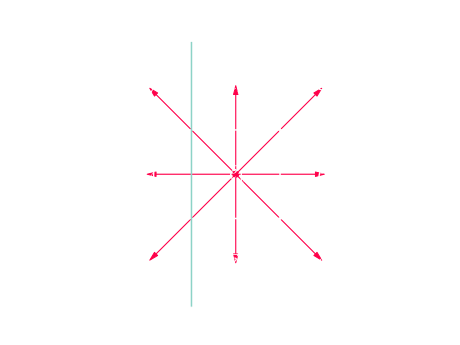
\includegraphics[width=\linewidth]{ei.pdf}
    \caption{Vitesses $\ei$ du réseau pour D2Q9.}
    \label{fig:ei}
  \end{figure}
  
  Il faut bien comprendre que nous aurions pu définir n'importe quel jeu de vitesses $\ei$ arbitraire\footnote{À partir du   
  moment où l'on respecte l'isotropie.}, tout comme on as choisi un jeu de positions $\r$ dans lequel notre simulation ce 
  déroulera, cette discrétisation dans l'espace des phases n'est fondamentalement pas beaucoup différent de ce que l'on
  fait plus couramment.
  
  Étant donnée la construction de notre réseau on peux définir la vitesse de maille $c$ :
  \begin{equation} \label{eq:c}
    c := \frac{\dl}{\dt}.
  \end{equation}
  
  A l'aide de la figure \ref{fig:ei} et de la définition de $c$ on peux définir les valeurs de $\ei$ pour notre 
  simulation:
  
  \begin{equation}
    \ei := c
    \begin{bmatrix}
      0&1&0&-1&0&1&-1&-1&1\\
      0&0&1&0&-1&1&1&-1&-1
    \end{bmatrix}.
  \end{equation}

  En utilisant la distribution de Maxwell-Boltzmann il nous est possible de calculer les poids $\w$ de la distribution à
  l'équilibre (et sans vitesse $\u$).
  Pour une LBM $D2Q9$ les poids $\w$ sont les suivants :
  
  \begin{equation}
    \w := \left[\frac{4}{9}; \frac{1}{9}; \frac{1}{9}; \frac{1}{9}; \frac{1}{9}; \frac{1}{36}; \frac{1}{36}; \frac{1}{36}; \frac{1}{36} \right],
  \end{equation}
  avec cette distribution a bien $\sum_{i=1}^Q \w = 1$.
  
  Précédemment nous avons dis que $c_s$ la vitesse du son était la vitesse moyenne $\left<||\v||\right>$ de nos particules.
  On peut donc écrire :
  
  \begin{equation}
    c_s^2 \delta_{\alpha \beta}= \sum_{i=1}^Q \w e_{i\alpha} e_{i\beta},
  \end{equation}
  appliqué au cas 2DQ9 cela nous donne :
  \begin{equation} \label{eq:cs}
    c_s = \frac{c}{\sqrt{3}}.
  \end{equation}
  
  Nous avons ainsi définie toutes les grandeurs dépendent de notre choix de $D2Q9$.
  
   
  \section{De l'équation de Boltzmann aux LBM (LBGK)}\label{seq:DiscB}
    \paragraph*{}
  Dans le cas que nous avons choisis nous pouvons réécrire l'équation de Boltzmann (\ref{eq:Bol})
  de la manière suivante :
  \begin{equation} \label{eq:BolnoF}
    \pderiv{f}{t} + \v \cdot \vnabla_{\r} f = C(f),
  \end{equation}
  si l'on remplace $C(f)$ par l'opérateur BGK :
  \begin{equation} \label{eq:BGK}
    C(f) = -\frac{1}{\tau}\left(f -\feq\right),
  \end{equation}
  on obtiens :
  \begin{equation} \label{eq:BolCF}
    \pderiv{f}{t} + \v \cdot \vnabla_{\r} f = -\frac{1}{\tau}\left(f -\feq\right).
  \end{equation}
  
  Si l'on ajoute $f$ des deux cotées et que l'on discrétise l'équation \ref{eq:BolCF} on obtiens notre résultat final :
  
  \begin{equation} \label{eq:LBGK}
    f_i(\r+\dt \ei, t + \dt) = f_i -\frac{1}{\tau}\left(f_i -\feq_i\right).
  \end{equation}
  
  Reste encore à définir les termes apparaissant dans notre équation,
  \begin{itemize} \label{eq:defmacro}
    \itemb $\tau$ :
      \begin{equation} \label{eq:tau}
        \tau = \frac{\nu}{c_s^2 \dt} + \frac{1}{2},
      \end{equation}
    \itemb $\feq_i$ :
      \begin{equation} \label{eq:feq}
        \feq_i = \w \rho \left(1 + \frac{\u \cdot \ei}{c_s^2} + \frac{(\u \cdot \ei)^2}{2 c_s^4} - \frac{\u \cdot \u}{2 c_s^2} \right),
      \end{equation}
      \itemb $\rho$ :
      \begin{equation} \label{eq:rho}
        \rho = \sum_{i=1}^Q f_i,
      \end{equation}
      \itemb $\u$ :
      \begin{equation} \label{eq:u}
        \u = \frac{1}{\rho}\sum_{i=1}^Q f_i\ei.
      \end{equation}
  \end{itemize}

  
  \section{Conditions aux bornes \& interactions}\label{seq:Bc}
    \paragraph*{}
  Nos équations décrivent notre fluide dans le domaine que nous avons défini mais ce n'est pas suffisant, il reste encore
  à définir comment notre fluide ce comporte aux frontières de notre domaine et comment il interagit avec notre domaine.
  
  En mécanique des fluides numérique il y as un jeu de condition aux bornes qui suffisent à décrire la majorité des   
  situations nous allons présenter ici celles que nous utiliserons dans nos simulations:
  
  \subsection{\bf Conditions périodiques :}
    Acclamé par la critique, les conditions périodiques aux bornes possèdent le bon goût d'être simples à implémenter et
    de ne présenter quasiment pas d'effet secondaire\footnote{Si ce n'est se placer dans un plan infini\dots}.
    
    \begin{figure}[hbtp]
      \centering
      \includegraphics[width=\linewidth]{periodic.pdf}
      \caption{Exemple de condition périodique matérialisée par les droites noires.}
      \label{fig:per}
    \end{figure}
  
    Dans ce cas il suffit de définir que les $f_i$ franchissant la frontière <<s'échangent>> avec leurs équivalents de
    la frontière rattaché, dans le cas de la figure \ref{fig:per} et avec les indices de la figure \ref{fig:ei} on peux     
    réécrire cela de manière plus formelle :
    
    $$
      \forall (\delta_x + \sign{e_{i,x}}) \in \Omega
    $$
    \begin{equation}     
      \begin{array}{rrcr}
        i \in [7,3,6] & f_i(\delta_x, 0) & \rightarrow & f_i(\delta_x + \sign{e_{i,x}}, 232),\\
        i \in [8,5,9] & f_i(\delta_x, 232) & \rightarrow & f_i(\delta_x + \sign{e_{i,x}}, 0),
      \end{array}
    \end{equation}
     avec $\Omega$ l'ensemble de la frontière considérée et $\sign{}$ la fonction qui renvoie le signe.



    \begin{figure}[hbtp]
      \centering
      \includegraphics[width=\linewidth]{iolet.pdf}
      \caption{Exemple de conditions d'entrée/sorties matérialisée par deux droites respectivement à gauche et à droite 
      du graphique.}
      \label{fig:iolet}    
    \end{figure}

  \subsection{\bf Entrée à vitesse imposée :}
    Quand il s'agit des entrées et de sorties il existe une référence dans le domaine et c'est l'article de
    Qisu Zou et Xiaoyi He\footnote{souvent abrégée en Zou \& He} \cite{Zou_1997}.
    Dans le cas de notre implémentation il nous à fallu les redémontrer dans le cadre des équations dimensionnées.
    
    L'idée est la suivante :
    Au niveau de l'entrée\footnote{Inlet en anglais (et dans la littérature en général).} dans le cas d'une entrée comme
    présentée dans la figure \ref{fig:iolet} après la diffusion $f_3, f_7, f_4, f_8, f_5$ son connus.
    On vas donc utiliser on les équations \ref{eq:rho} et \ref{eq:u} pour déterminer les inconnues $f_6, f_2, f_9$ et 
    $\rho$, si l'on écris explicitement les sommes des équations \ref{eq:rho} et \ref{eq:u} pour notre simulation $D2Q9$ 
    on obtiens :
    $$
      \rho = f_1 + f_2 + f_3 + f_4 + f_5 + f_6 + f_7 + f_8 + f_9,
    $$
    $$
      \rho u_x = c(f_2 - f_4 + f_6 - f_7 - f_8 + f_9),
    $$
    $$
      \rho u_y = c(f_3 - f_5 + f_6 + f_7 - f_8 - f_9).
    $$
     
    On peux réécrire ces équations pour faire apparaitre les $f_i$ inconnue d'un coté et les autres termes de l'autre :
    \begin{equation} \label{eq:zhrho}
      f_6 + f_2 + f_9 = \rho - (f_1 + f_3 + f_4 + f_5 + f_7 + f_8),
    \end{equation}      
    \begin{equation} \label{eq:zhux}
      f_6 + f_2 + f_9 = \frac{\rho u_x}{c} + ( f_4 + f_7 + f_8),
    \end{equation}
    \begin{equation} \label{eq:zhuy}
      f_6 - f_9 = \frac{\rho u_y}{c} - (f_3 - f_5 + f_7 - f_8).
    \end{equation}
    
    En soustrayant les equations \ref{eq:zhrho} et \ref{eq:zhux} et en réarrangeant les termes on obtiens :
    \begin{equation} \label{eq:rhozh}
      \rho = \frac{c}{c - u_x}(f_1 + f_3 + f_5 + 2( f_4 + f_7 + f_8)),
    \end{equation}
    étant donnée que l'on impose la vitesse $\u$ sur l'inlet l'équation \ref{eq:rhozh} nous donne la valeur de 
    l'inconnue $\rho$. Pour poursuivre le raisonnement il faut faire l'hypothèse\footnote{C'est là ou ce trouve le 
    <<tour de force>> de l'article \cite{Zou_1997}} que $f_2 - \feq_2 = f_4 - \feq_4$.
    Si l'on développe avec l'équation \ref{eq:feq} et \ref{eq:cs} cette hypothèse et que l'on simplifie on obtiens:    
    \begin{equation} \label{eq:f2zh}
      f_2 = f_4 + \frac{2\rho u_x}{3c}.
    \end{equation}
    Si l'on remplace \ref{eq:f2zh} dans \ref{eq:zhux} on obtiens :
    \begin{equation} \label{eq:f69zh}
      f_6 + f_9 =  \frac{\rho u_x}{3c} + f_7 + f_8,
    \end{equation}
    en sommant l'équation \ref{eq:f69zh} avec \ref{eq:zhuy} et en simplifiant on obtiens :
    \begin{equation} \label{eq:f6zh}
      f_6 =  f_8 + \frac{\rho}{2c}\left(\frac{u_x}{3} + u_y\right) + \frac{1}{2}(f_5 - f_3),
    \end{equation}
    la même chose en soustrayant l'équation \ref{eq:f69zh} avec \ref{eq:zhuy} et en simplifiant on obtiens :
    \begin{equation} \label{eq:f6zh}
      f_9 =  f_7 + \frac{\rho}{2c}\left(\frac{u_x}{3} - u_y\right) + \frac{1}{2}(f_3 - f_5),
    \end{equation}
    dans le cas d'un écoulement incompressible on peut prendre $\rho = 1$ ce qui permet encore de simplifier nos 
    équations.  
    Nous avons donc notre jeux d'équations suivant pour notre entrée :
    \begin{equation} \label{eq:vinlet}  
      \begin{array}{rcl}
        f_2 &=& f_4 + 2\dfrac{u_x}{3c},\\
        f_6 &=&  f_8 + \dfrac{1}{2}\left(\dfrac{u_x}{3c} + \dfrac{u_y}{c} + f_5 - f_3\right),\\
        f_9 &=&  f_7 + \dfrac{1}{2}\left(\dfrac{u_x}{3c} - \dfrac{u_y}{c} + f_3 - f_5\right).
      \end{array}
    \end{equation}
    
    \subsection{\bf Sortie à pression imposée :}
      Pour la sortie on suppose que $u_y = 0$ et que $\rho = \rho_\text{out}$, il nous reste à trouver les valeurs de 
      $u_x$ ainsi que de $f_7, f_4, f_8$ (dans le cas de la figure \ref{fig:iolet}).
      Avec le même raisonnement que précédemment et avec \ref{eq:rho} et \ref{eq:u} on obtiens :
      \begin{equation} \label{eq:zhorho}
        f_7 + f_4 + f_8 = \rho_\text{out} - (f_1 + f_2 + f_3 + f_5 + f_6 + f_9),
      \end{equation}      
      \begin{equation} \label{eq:zhoux}
        f_7 + f_4 + f_8 = \frac{\rho_\text{out} u_x}{c} + ( f_2 + f_6 + f_9),
      \end{equation}
      \begin{equation} \label{eq:zhouy}
        f_7 - f_8 = - f_3 + f_5 - f_6 + f_9.
      \end{equation}
      En soustrayant les equations \ref{eq:zhorho} et \ref{eq:zhoux} et en réarrangeant les termes on obtiens :
      \begin{equation} \label{eq:uxzh}
        u_x = c - \frac{c}{\rho_\text{out}}(f_1 + f_3 + f_5 + 2( f_6 + f_2 + f_9)),
      \end{equation}
      étant donnée que l'on impose la densité $\rho_\text{out}$ sur l'outlet l'équation \ref{eq:uxzh} nous donne la 
      valeur de l'inconnue $u_x$. 
      En réutilisant la même hypothèse et la même méthode que précédemment on obtiens :
      \begin{equation} \label{eq:f4zh}
        f_4 = f_2 + \dfrac{2\rho_\text{out} u_x}{3c},
      \end{equation}
      \begin{equation} \label{eq:f7zh}
        f_7 = f_9 + \dfrac{1}{2}\left( \dfrac{\rho_\text{out} u_x}{3c} + f_5 - f_3 \right),
      \end{equation}
      \begin{equation} \label{eq:f8zh}
        f_8 = f_6 + \dfrac{1}{2}\left(\dfrac{\rho_\text{out} u_x}{3c} + f_3 - f_5 \right).
      \end{equation}
      La encore dans le cas d'un écoulement incompressible on peut prendre $\rho_\text{out} = 1$ ce qui permet de 
      simplifier nos équations.  
      Nous avons donc notre deuxième jeux d'équations suivant pour notre sortie:
      \begin{equation} \label{eq:poutlet}  
        \begin{array}{rcl}
          u_x &=& c(1 - [f_1 + f_3 + f_5 + 2( f_6 + f_2 + f_9)]),\\
          f_4 &=& f_2 + \dfrac{2 u_x}{3c},\\
          f_7 &=& f_9 + \dfrac{1}{2}\left( \dfrac{u_x}{3c} + f_5 - f_3 \right),\\
          f_8 &=& f_6 + \dfrac{1}{2}\left(\dfrac{u_x}{3c} + f_3 - f_5 \right).
        \end{array}
      \end{equation}

    \begin{figure}[hbtp]
      \centering
      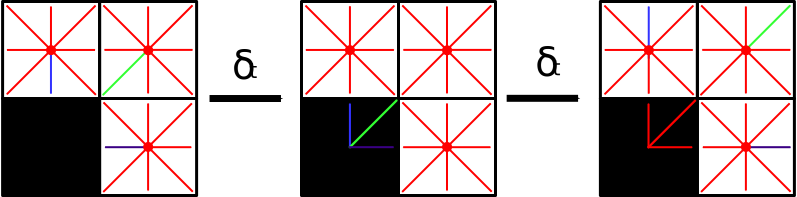
\includegraphics[width=\linewidth]{Fig/collide.pdf}
      \caption{Illustration du processus de collision avec un object (en noir).}
    \end{figure}     
    \subsection{\bf collision sans glissement :}

      Avec tout ce dons nous venons de discuter jusqu'ici il est évident que nous allons étudier un flux\footnote{Flow 
      Driven Analyses dans la littérature.}, mais pour l'instant nous n'avons pas encore discuté de l'interaction entre
      notre fluide et autre chose que lui-même.
      Les collisions sans glissement\footnote{Aussi appelées <<no slip boundaries>>.} peuvent s'interpréter de la 
      manière suivante : étant donnée une population de particules $f_i$ associée à une vitesse microscopique $\ei$ qui 
      rentre en collision avec un solide, elle va rebondir et repartir avec une vitesse $\ei$ opposée.
      Autrement dis pour simuler une collision il suffit d'échanger les populations $f_i$ de particules entre les 
      vitesses correspondante.
      Si l'on ce réfère à la figure \ref{fig:ei} nous avons les échanges suivants :
      \begin{equation}     
        \begin{array}{rcr}
          f_2 & \leftrightharpoons & f_4,\\
          f_3 & \leftrightharpoons & f_5,\\
          f_6 & \leftrightharpoons & f_8,\\
          f_7 & \leftrightharpoons & f_9,\\
        \end{array}
      \end{equation}
      $f_1$ correspondant aux particules au repos n'est pas échangé.
      

      
      

  \section{Algorithme \& implémentation}\label{seq:Al&i}
    \paragraph*{}
  Il est désormais temps d'implémenter notre LBM, l'algorithme ce décompose en trois étapes :
  \begin{itemize} \label{eq:defmeso}
    \itemb Initialisation :\\
    \emph{On définie les valeurs aux bornes et l'on applique les rebond sur les objets (on échange les populations).}
    \itemb Flux :\\
    \emph{On déplace les populations de $\ei \dt$.}
    \itemb Collision :\\
    \emph{On applique l'opérateur collision sur les populations $f_i$.}  
  \end{itemize}
  On répète ces étapes en boucle pour simuler le comportement du fluide.
  
  \begin{figure}[hbtp]
    \centering
    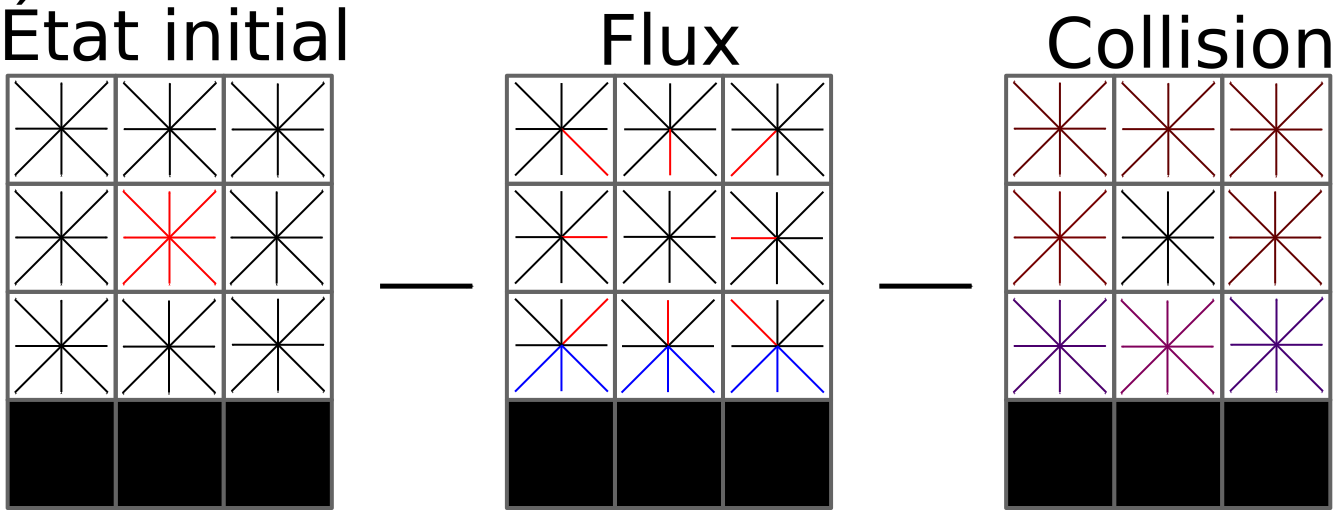
\includegraphics[width=\linewidth]{Fig/algorithme.pdf}
    \caption{Shéma des différentes étapes de résulotion de la LBM.}
  \end{figure}
  
   Cette structure est effectivement bien visible dans notre code {\sc Fortran}:
  \begin{minted}{fortran}
!===============================================================================
!                               The main program.
!===============================================================================
Program LBM2D
  Use Var
  Use Dconst, Only: L, H, N
  Implicit None
  Integer(4) :: dN, d = 100, ni = 0
  Call Allocatall             ! Alloue les variables en mémoire
  Call InitF                  ! Initialise les variables
  
  Do dN = 0, N
    If (Modulo(dN, d) == 0) Then      
      Call Savefile(ni)      ! Sauvegarde les valeurs intermédiaires pour pouvoir faire des animations
      ni = ni + 1
    End If

    CALL IOlet                ! Initialisation
    CALL Bound                ! Initialisation
    CALL Stream               ! Flux
    CALL CMacro               ! Collision : calcul les valeurs macro
    CALL CFeq                 ! Collision : calcul les valeurs de feq
    CALL Collide              ! Collision : applique l'opérateur collision
  End Do
  
  Call Deallocatall           ! Libère la mémoire
End Program LBM2D
  \end{minted}
  
  durant l'implémentation nous avons fait le choix d'utiliser des subroutines afin de minimiser l'impact mémoire (La 
  gestion de la mémoire est un problème critique dans notre code nous avons donc privilégié le passage par référence 
  plutôt que le passage par valeur).
  De plus pour accélérer notre code nous avons utilisée énormément de boucles Do en respectant l'ordre des indices,
  comme par exemple dans la subroutine collide :
  \begin{minted}{fortran}
!===============================================================================
!                             Collide Step
!===============================================================================
Subroutine Collide
  Use Var, Only: F, Feq
  Use Cconst, Only: itau, mitau
  Use Dconst, Only: L, H
  Use Lconst, Only: Q
  Implicit None
  Integer(4) :: i, j
  Integer(1) :: k
  
  Do j = 1, H
    Do i = 1, L
      Do k = 1, Q
        F(k,i,j)= mitau*F(k,i,j) + itau*Feq(k,i,j)
      End Do
    End Do
  End Do
End Subroutine
  \end{minted}
    cette subroutine est l'implémentation de l'équation \ref{eq:LBGK}.
  
  
  
  \section{Premiers tests et écoulements indépendant du temps.}
    Notre étude ce porteras dans un premier temps à vérifier que notre implémentation de LBM concorde avec la théorie.
Pour cela nous allons étudier l'écoulement de Poiseuille nous allons donc placer un profil en forme de tube dans notre simulation. Pour vérifier la corrélation avec les résultats théorique nous allons intégrer le débit volumique à deux
niveau et on vas pouvoir ainsi vérifier la conservation du débit volumique.
En plus nous avons la formule théorique de l'écoulement de Poiseuille 

\begin{equation}
  v(z) = v_\text{max} \left(\frac{4z}{h} - \frac{4z^2}{h^2}\right),
\end{equation}

en intégrant sur $h$ on obtiens $v_\text{max}$ en fonction du débit volumique $D_v$ : 

\begin{equation}
  D_v = v_\text{max} \frac{2h}{3}.
\end{equation}

Étant donné que notre écoulement et incompressible en intégrant numériquement sur une première section on obtiens donc 
le profil de vitesse pour la deuxième section :

\begin{equation}
  v(x) = D_v \frac{3}{2h} \left( \frac{4z}{h} - \frac{4z^2}{h^2} \right).
\end{equation}

Voici les différents résultats obtenus :

\begin{figure}[hbtp]
  \centering
  \includegraphics[width=\linewidth]{Fig/Poiseuille.png}
  \caption{Étude de l'écoulement de Poiseuille dans un cas simple}
  \label{fig:P1}
\end{figure}
On observe que le débit volumique et conservée (à l'équilibre) de plus le profil des vitesse simulé colle parfaitement 
à la théorie. 
\begin{figure}[hbtp]
  \centering
  \includegraphics[width=\linewidth]{Fig/Poiseuille2.png}
  \caption{Étude de l'écoulement de Poiseuille dans une géométrie plus complexe}
  \label{fig:P2}
\end{figure}
\begin{figure}[hbtp]
  \centering
  \includegraphics[width=\linewidth]{Fig/Poiseuille3.png}
  \caption{Étude de l'écoulement de Poiseuille dans une géométrie encore un peu plus complexe}
  \label{fig:P3}
\end{figure}

On observe pour la figure \ref{fig:P2} une nouvelle fois un très bon accord avec la théorie le débit volumique est toujours conservé. À partir de la figure \ref{fig:P3} le profil des vitesses ne colle plus totalement à la théorie, rien de très inquiétant étant donné que ce profile sort du domaine de définition de la théorie de poiseuille néanmoins le débit volumique et toujours conservé. 

Maintenant que nous avons confirmé que notre simulation concordais avec la théorie, nous pouvons essayer de simuler des 
systèmes non solvables analytiquement comme pour la figure \ref{fig:CF}. 

\begin{figure}[hbtp]
  \centering
  \includegraphics[width=\linewidth]{Fig/CF.png}
  \caption{Étude de l'écoulement dans une géométrie complexe}
  \label{fig:CF}
\end{figure}

La méthode lattice Boltzmann s'adapte donc bien à des géométries variées, et le débit volumique est toujours conservée.
Mais jusqu'à présent nous n'avons fait qu'étudier des flux qui converge vers des solutions indépendantes du temps.

  
  \section{Solutions périodiques et allée de tourbillons de Von Karman.}
    Dans le but de pousser notre implémentation de la LBM un peu plus loin, nous avons simulée le flux autour d'une aile d'avion, le but était d'obtenir nos premiers écoulements dépendant du temps, voici en figure \ref{fig:VK} un des résultat que nous avons obtenu.

\begin{figure}[hbtp]
  \centering
  \includegraphics[width=\linewidth]{Fig/VK.png}
  \caption{Allée de Von Karman pour $Re \approx 400$}
  \label{fig:VK}
\end{figure}

Afin d'étudier plus quantitativement nos résultats nous avons choisi deux points d'intérêt au niveau de l'allée de Von Karman et nous avons tracée la trajectoire dans l'espace des phases de ces points, passée un régime de transition, ces trajectoires convergeaient vers une orbite périodique. L'analyse de la trajectoire dans l'espace des phases est un outil
très puissant quand il es question de caractériser les écoulements auquel nous avons à faire.
Très vite lors de nos simulations nous avons systématiquement utilisé le nombre de Reynolds afin de pouvoir avoir une idée avant de lancer la simulation de la physique que nous allions avoir.


    
  \section{Solution chaotiques}
    Dans un derniers effort nous avons poussée notre simulation vers les haut nombres de Reynolds, nous avons pu observer des 
comportements chaotiques. Là encore nos visualisation nous on permis de quantifier ce comportement.

\begin{figure}[hbtp]
  \centering
  \includegraphics[width=\linewidth]{Fig/little_chaos.png}
  \caption{Rotationnel d'un écoulement chaotique $Re \approx 1000$}
  \label{fig:lChaos}
\end{figure}

Les comportements chaotiques sont très riches et nous aurions aimé plus étudier ces simulation malheureusement ces simulations arrievent à la limite de ce qui est faisable techniquement avec le matériel à notre disposition.\footnote{les simulations des figures \ref{fig:lChaos} et \ref{fig:VK} on nécessité chacune plus de 120 Go de stockage et plus de 6h de simulations.}
\begin{figure}[hbtp]
  \centering
  \includegraphics[width=\linewidth]{Fig/chaos.pdf}
  \caption{Rotationnel d'un écoulement chaotique $Re \approx 4000$}
  \label{fig:Chaos}
\end{figure}
  
  \section{Conclusion}
    Dans le cadre de ce projet, nous avons pu implémenter la méthode de Boltzmann sur réseau, ce fut une aventure très riche
et surtout très intéressante.
Les résultats obtenus prouvent la polyvalence de la méthode pour simuler de nombreux systèmes.
La méthode lattice Boltzmann ne bénéficie pas encore d'une documentation claire, ni standardisée, ni rigoureuse\footnote{En tout cas si elle existe elle n'est pas disponible.}  
ce qui peut être très frustrant quand on cherche de la documentation sur le sujet. Il faut garder en tête que c'est un domaine relativement récent. Est il constitue un domaine de recherche très actif.
Les LBM peuve implémenter bien plus que seulement la physique des fluide et nous aurions aimées implémenter de la thermodynamiques et des interactions entre deux fluide mais le temps et la contingence ne nous ont pas permis d'aller aussi loin que souhaité mais la fin de ce projet ne marque pas la fin de ce travail. le \href{https://github.com/Pacidus/LBM_project}{github associé à ce projet} resteras actif encore pour un moment, avec même un \href{https://pacidus.github.io/LBM_project/}{site web associé} en cours de développement. 
  
  \vfill  
  \newpage
  \vfill

  \bibliographystyle{unsrt}
  \bibliography{bibLBM}
    
 
%\begin{biography}{}{\author{Yohan Duarte} Biography text}
%\end{biography}
  \vfill
  \newpage

  \vspace{10cm}

  \onecolumn
  \section{Code {\sc Fortran}}
    \inputminted{fortran}{Codes/windtunnel.f90}
  
  \vfill
  \newpage
  \section{Code {\sc Python} pour les animations et l'analyse des données}
    \section{Animation fluide}
      \inputminted{python}{Codes/anim.py}
    
    \vfill
    \newpage
    \section{Animation analyse Poiseuille}
      \inputminted{python}{Codes/sprofile.py}

    \vfill
    \newpage    
    \section{Animation analyse Von Karmann}
      \inputminted{python}{Codes/interesting.py}
      
    \vfill
    \newpage   
    \section{Automatisation et animations}
      \inputminted{makefile}{Codes/makefile}
\end{document}